% \documentclass[table]{beamer}
\documentclass[table,handout]{beamer}
\setbeameroption{show notes}
% \setbeameroption{hide notes}
% \setbeameroption{show only notes}
\usepackage{varwidth}

\newif\ifhide
\newif\ifpost
\newif\ifhideclicker

% \hidetrue
% \hideclickertrue
% \posttrue

\newcommand{\whiteout}[1]{\textcolor{white}{#1}}
% \newcommand{\whiteoutbox}[1]{\fcolorbox{white}{white}{\parbox{\dimexpr \linewidth-2\fboxsep-2\fboxrule}{\whiteout{#1}}}}
% \newcommand{\notebox}[1]{\fcolorbox{blue}{white}{\parbox{\dimexpr \linewidth-2\fboxsep-2\fboxrule}{#1}}}
\newcommand{\whiteoutbox}[1]{\fcolorbox{white}{white}{\parbox{\linewidth}{\whiteout{#1}}}}
\newcommand{\notebox}[1]{\fcolorbox{blue}{white}{\parbox{\linewidth}{#1}}}
\newcommand{\blankbox}[1]{\phantom{\varwidth{\linewidth}\whiteoutbox{#1}\endvarwidth}}
\newcommand{\blank}[1]{\phantom{\varwidth{\linewidth}#1\endvarwidth}}

\ifhide%
    \newcommand{\hmask}[1]{\blank{#1}}%
\else%
    \newcommand{\hmask}[1]{#1}%
\fi

\ifhide%
    \newcommand{\wout}[1]{\whiteout{#1}}%
\else%
    \newcommand{\wout}[1]{#1}%
\fi

\ifhide%
    \newcommand{\hignore}[1]{}%
\else%
    \newcommand{\hignore}[1]{#1}%
\fi

\ifpost%
    \newcommand{\nopost}[1]{}%
\else%
    \newcommand{\nopost}[1]{#1}%
\fi

\ifhideclicker%
    \newcommand{\clickerslide}[1]{\stepcounter{clickerQuestionCounter}%
        \begin{frame}[t]
            \textcolor{blue}{Q \arabic{clickerQuestionCounter}:}
        \end{frame}}
\else%
    \newcommand{\clickerslide}[1]{#1}%
\fi

\ifhide%
    \newcommand{\hidebox}[1]{\blank{#1}}%
\else%
    \newcommand{\hidebox}[1]{\notebox{#1}}%
\fi

\ifhide%
    \newcommand{\wbox}[1]{\whiteoutbox{#1}}%
\else%
    \newcommand{\wbox}[1]{\notebox{#1}}%
\fi

\ifhide%
    \newcommand{\nbox}[1]{\blankbox{#1}}%
\else%
    \newcommand{\nbox}[1]{\notebox{#1}}%
\fi

\ifhideclicker%
    \newcommand{\clickeranswer}[1]{#1}%
\else%
    \ifhide%
        \newcommand{\clickeranswer}[1]{#1}%
    \else%
        \newcommand{\clickeranswer}[1]{\textbf{\textcolor{blue}{#1}}}%
    \fi
\fi

\usepackage{beamerthemesplit}
% \usetheme{boxes}
\usetheme{Malmoe}
\usecolortheme{seahorse}
% \usecolortheme{seagull}
\usepackage{ifthen}
\usepackage{xspace}
\usepackage{multirow}
\usepackage{multicol}
\usepackage{booktabs}
\usepackage{xcolor}
\usepackage{wasysym}
\usepackage{comment}
\usepackage{hyperref}
\hypersetup{pdfborder={0 0 0}, colorlinks=true, urlcolor=blue, linkcolor=blue, citecolor=blue}
\usepackage{changepage}
\usepackage[compatibility=false]{caption}
\captionsetup[figure]{font=scriptsize, labelformat=empty, textformat=simple, justification=centering, skip=2pt}
\usepackage{tikz}
\usetikzlibrary{trees,calc,backgrounds}

\usepackage[bibstyle=joaks-slides,maxcitenames=3,mincitenames=1,backend=biber]{biblatex}

\newrobustcmd*{\shortfullcite}{\AtNextCite{\renewbibmacro{title}{}\renewbibmacro{in:}{}\renewbibmacro{number}{}}\fullcite}

\newrobustcmd*{\footlessfullcite}{\AtNextCite{\renewbibmacro{title}{}\renewbibmacro{in:}{}}\footfullcite}

% Make all footnotes smaller
% \renewcommand{\footnotesize}{\scriptsize}

\definecolor{myGray}{gray}{0.9}
\colorlet{rowred}{red!30!white}

\setbeamertemplate{blocks}[rounded][shadow=true]

\setbeamercolor{defaultcolor}{bg=structure!30!normal text.bg,fg=black}
\setbeamercolor{block body}{bg=structure!30!normal text.bg,fg=black}
\setbeamercolor{block title}{bg=structure!50!normal text.bg,fg=black}

\newenvironment<>{varblock}[2][\textwidth]{%
  \setlength{\textwidth}{#1}
  \begin{actionenv}#3%
    \def\insertblocktitle{#2}%
    \par%
    \usebeamertemplate{block begin}}
  {\par%
    \usebeamertemplate{block end}%
  \end{actionenv}}

\newenvironment{displaybox}[1][\textwidth]
{
    \centerline\bgroup\hfill
    \begin{beamerboxesrounded}[lower=defaultcolor,shadow=true,width=#1]{}
}
{
    \end{beamerboxesrounded}\hfill\egroup
}

\newenvironment{onlinebox}[1][4cm]
{
    \newbox\mybox
    \newdimen\myboxht
    \setbox\mybox\hbox\bgroup%
        \begin{beamerboxesrounded}[lower=defaultcolor,shadow=true,width=#1]{}
    \centering
}
{
    \end{beamerboxesrounded}\egroup
    \myboxht\ht\mybox
    \raisebox{-0.25\myboxht}{\usebox\mybox}\hspace{2pt}
}

\newenvironment{mydescription}{
    \begin{description}
        \setlength{\leftskip}{-1.5cm}}
    {\end{description}}

\newenvironment{myitemize}{
    \begin{itemize}
        \setlength{\leftskip}{-.3cm}}
    {\end{itemize}}

% footnote without a marker
\newcommand\barefootnote[1]{%
  \begingroup
  \renewcommand\thefootnote{}\footnote{#1}%
  \addtocounter{footnote}{-1}%
  \endgroup
}

% define formatting for footer
\newcommand{\myfootline}{%
    {\it
    \insertshorttitle
    \hspace*{\fill} 
    \insertshortauthor, \insertshortinstitute
    % \ifx\insertsubtitle\@empty\else, \insertshortsubtitle\fi
    \hspace*{\fill}
    \insertframenumber/\inserttotalframenumber}}

% set up footer
\setbeamertemplate{footline}{%
    \usebeamerfont{structure}
    \begin{beamercolorbox}[wd=\paperwidth,ht=2.25ex,dp=1ex]{frametitle}%
        % \Tiny\hspace*{4mm}\myfootline\hspace{4mm}
        \tiny\hspace*{4mm}\myfootline\hspace{4mm}
    \end{beamercolorbox}}

% remove navigation bar
\beamertemplatenavigationsymbolsempty

\makeatletter
    \newenvironment{noheadline}{
        \setbeamertemplate{headline}[default]
        \def\beamer@entrycode{\vspace*{-\headheight}}
    }{}
\makeatother

\newcounter{clickerQuestionCounter}
\ifhideclicker%
\newenvironment{clickerquestion}
{ \stepcounter{clickerQuestionCounter}
  \begin{enumerate}[Q \arabic{clickerQuestionCounter}:]\color{white} }
{ \end{enumerate} }
\else%
\newenvironment{clickerquestion}
{ \stepcounter{clickerQuestionCounter}
  \begin{enumerate}[Q \arabic{clickerQuestionCounter}:] }
{ \end{enumerate} }
\fi

\ifhideclicker%
\newenvironment{clickeroptions}
{ \begin{enumerate}[\begingroup\color{white} 1)\endgroup]\color{white} }
{ \end{enumerate} }
\else%
\newenvironment{clickeroptions}
{ \begin{enumerate}[\begingroup\color{red} 1)\endgroup] }
{ \end{enumerate} }
\fi


\tikzstyle{centered} = [align=center, text centered, font=\sffamily\bfseries]
\tikzstyle{skip} = [centered, inner sep=0pt, fill]
\tikzstyle{empty} = [centered, inner sep=0pt]
\tikzstyle{inode} = [centered, circle, minimum width=4pt, fill=black, inner sep=0pt]
\tikzstyle{tnode} = [centered, circle, inner sep=1pt]
\tikzset{
  % edge styles
  level distance=10mm,
  mate/.style={edge from parent/.style={draw,distance=3pt}},
  mleft/.style={grow=left, level distance=10mm, edge from parent path={(\tikzparentnode.west)--(\tikzchildnode.east)}},
  mright/.style={grow=right, level distance=10mm, edge from parent path={(\tikzparentnode.east)--(\tikzchildnode.west)}},
  % node styles
  male/.style={rectangle,minimum size=4mm,fill=gray!80},
  female/.style={circle,minimum size=4mm,fill=gray!80},
  amale/.style={male,fill=red},
  afemale/.style={female,fill=red},
}

\newcommand{\highlight}[1]{\textcolor{violet}{\textit{\textbf{#1}}}}
\newcommand{\super}[1]{\ensuremath{^{\textrm{\sffamily #1}}}}
\newcommand{\sub}[1]{\ensuremath{_{\textrm{\sffamily #1}}}}
\newcommand{\dC}{\ensuremath{^\circ{\textrm{C}}}}
\newcommand{\tb}{\hspace{2em}}
\providecommand{\e}[1]{\ensuremath{\times 10^{#1}}}
\newcommand{\myHangIndent}{\hangindent=5mm}

\newcommand{\spp}[1]{\textit{#1}}

\newcommand\mybullet{\leavevmode%
\usebeamertemplate{itemize item}\hspace{.5em}}

\makeatletter
\newcommand*{\rom}[1]{\expandafter\@slowromancap\romannumeral #1@}
\makeatother

\newcommand{\blankslide}{{\setbeamercolor{background canvas}{bg=black}
\setbeamercolor{whitetext}{fg=white}
\begin{frame}<handout:0>[plain]
\end{frame}}}

\newcommand{\whiteslide}{
\begin{frame}<handout:0>[plain]
\end{frame}}

\newcommand{\f}[1]{\ensuremath{F_{#1}}}
\newcommand{\x}[1]{X\ensuremath{^{#1}}}
\newcommand{\y}[1]{Y\ensuremath{^{#1}}}

% Population growth macros
\newcommand{\popsize}[1]{\ensuremath{N_{#1}}}
\newcommand{\popgrowthratediscrete}[1]{\ensuremath{\lambda_{#1}}}
\newcommand{\popgrowthrate}[1]{\ensuremath{r_{#1}}}
\newcommand{\ptime}{\ensuremath{t}\xspace}

\tikzset{hide on/.code={\only<#1>{\color{white}}}}
\tikzset{
    invisible/.style={opacity=0},
    visible on/.style={alt={#1{}{invisible}}},
    alt/.code args={<#1>#2#3}{%
        \alt<#1>{\pgfkeysalso{#2}}{\pgfkeysalso{#3}}
        % \pgfkeysalso doesn't change the path
    },
}

\bibliography{../bib/references}
\author[J.\ Oaks]{
    %Jamie R.\ Oaks\inst{1}
    Jamie R.\ Oaks
}
\institute[BIOL 180]{
    \inst{}%
        BIOL 180: Introductory Biology
}



\title[Consumption]{Consumption}
% \date{\today}
\date{May 21, 2015}

% \setbeamertemplate{section in toc}[sections numbered]
% \setbeamertemplate{subsection in toc}[subsections numbered]

\begin{document}

\begin{noheadline}
\maketitle
\end{noheadline}

\nopost{
\begin{noheadline}
\begin{frame}[c]
    \vspace{-6mm}
    \begin{center} 
        \includegraphics[height=1.2\textheight]{../images/seating-chart-2.pdf}
    \end{center}
\end{frame}
\end{noheadline}
}

\begin{noheadline}
\begin{frame}
\frametitle{Today's issues:}
\vspace{5mm}
% \tableofcontents[subsectionstyle=hide]
\tableofcontents
\end{frame}
\end{noheadline}

\section{How does predation affect prey populations?}

\begin{frame}[t]
    \begin{adjustwidth}{-2em}{-1.5em}
        \vspace{-3mm}
        How does predation affect prey populations?

        \vspace{2mm}
        Question: Do predators reduce prey populations below the level that can
        be supported by available resources?

        \vspace{2mm}
        \begin{uncoverenv}<2->
        Predator removal experiments:
        \begin{itemize}
            \item Wolves and cougars removed from the Kaibab Plateau, 1907--1937

            \vspace{2mm}
            \item Start:
                
                \nbox{$\approx$4000 deer}

            \vspace{1mm}
            \item 1920:
                
                \nbox{$\approx$100,000 deer}

        \end{itemize}
        \end{uncoverenv}

        \begin{uncoverenv}<3->
        \vspace{2mm}
        Does this support the hypothesis that predators control prey
        populations?

        \nbox{\scriptsize Yes, this rapid increase of deer after removing
            predators is strong evidence of top-down control of prey
            populations by predators}

        What happened to habitat after deer density exploded?

        \nbox{\scriptsize Deer browse shrubs and small trees---stripped
            vegetation and compacted soil; population crashed}

        \end{uncoverenv}

    \end{adjustwidth}
    \note[item]{Classic way to test this is by removing or adding
        predators; with/without experiment}
    \note[item]{Kaibab Plateau, Arizona. Federal and state government paid
        people to kill top predators}
\end{frame}

\begin{frame}[t]
    \begin{adjustwidth}{-2em}{-1.5em}
        \vspace{-3mm}
        Predator addition experiments: Restoring wolves to the Yellowstone
        ecosystem

        \begin{uncoverenv}<2->
        \begin{columns}

        \column{0.5\linewidth}

        \vspace{2mm}
        Wolves were extirpated in the 1920s and reintroduced in 1995; elk are
        their main prey.

        % \vspace{2mm}
        \begin{enumerate}
            \item What is the graph's take-home message?

                \nbox{Elk reproduction PER FEMALE is reduced when wolves are
                    present.}

            \item Create a hypothesis to explain the data.

                \nbox{\scriptsize Females are expending time and energy
                    avoiding wolves, and have less energy to invest in
                    reproduction.}
        \end{enumerate}

        \column{0.49\linewidth}

        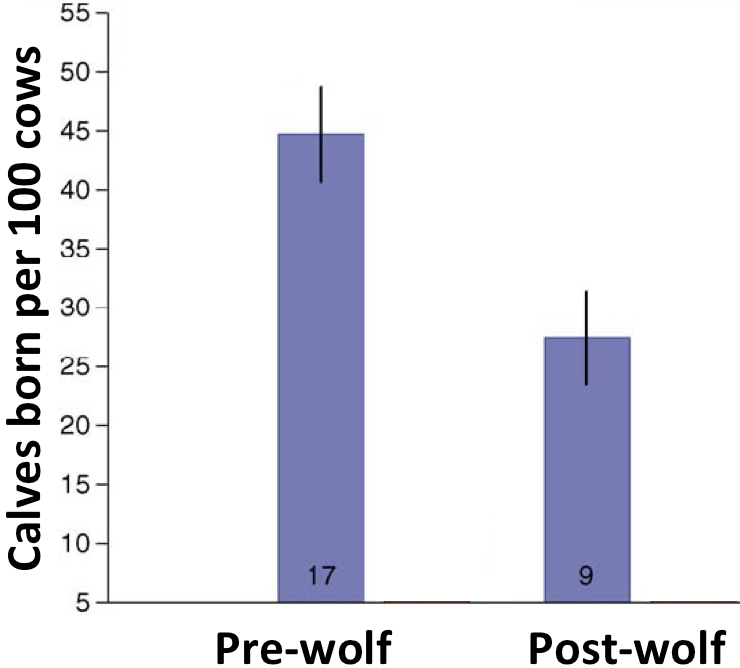
\includegraphics[width=\columnwidth]{elk.png}

        \end{columns}
        \end{uncoverenv}

    \end{adjustwidth}
    \note[item]{Note: Numbers at base of bars are the number of herds sampled}
\end{frame}

\clickerslide{
\begin{frame}
    \begin{adjustwidth}{-2em}{-1.5em}
        \begin{columns}

            \column{0.5\linewidth}

            \begin{clickerquestion}
                \item Which of the following is the best interpretation of this graph?
                \begin{clickeroptions}
                    \item \clickeranswer{The proportion of elk that are
                            vigilant is greatest when wolves are near.}
                    \item Vigilance is a heritable trait that can evolve. 
                    \item Females are more vigilant than males.
                    \item Elk aren't vigilant unless wolves are near. 
                \end{clickeroptions}
            \end{clickerquestion}

            \column{0.5\linewidth}

            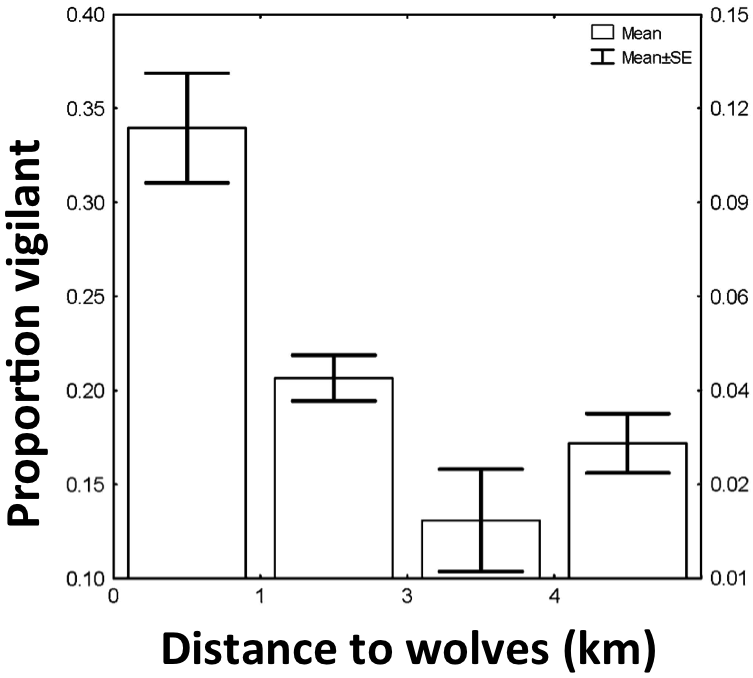
\includegraphics[width=\columnwidth]{elk-vigilance.png}

        \end{columns}

        \vspace{2mm}
        How does this connect to the observation in the previous graph?

    \end{adjustwidth}
\end{frame}
}

\clickerslide{
\begin{frame}
    \begin{adjustwidth}{-2em}{-1.5em}
        \begin{columns}

            \column{0.45\linewidth}

            \begin{clickerquestion}
                \item Which of the following is the best interpretation of this graph?
                \begin{clickeroptions}
                    \item Testosterone makes you stupid. 
                    \item Elk vigilance varies with distance to wolves.
                    \item Cows and bulls are equally vigilant when wolves are
                        absent or present.
                    \item \clickeranswer{Cows are more vigilant when wolves are
                            present; males show no difference.} 
                \end{clickeroptions}
            \end{clickerquestion}

            \column{0.55\linewidth}

            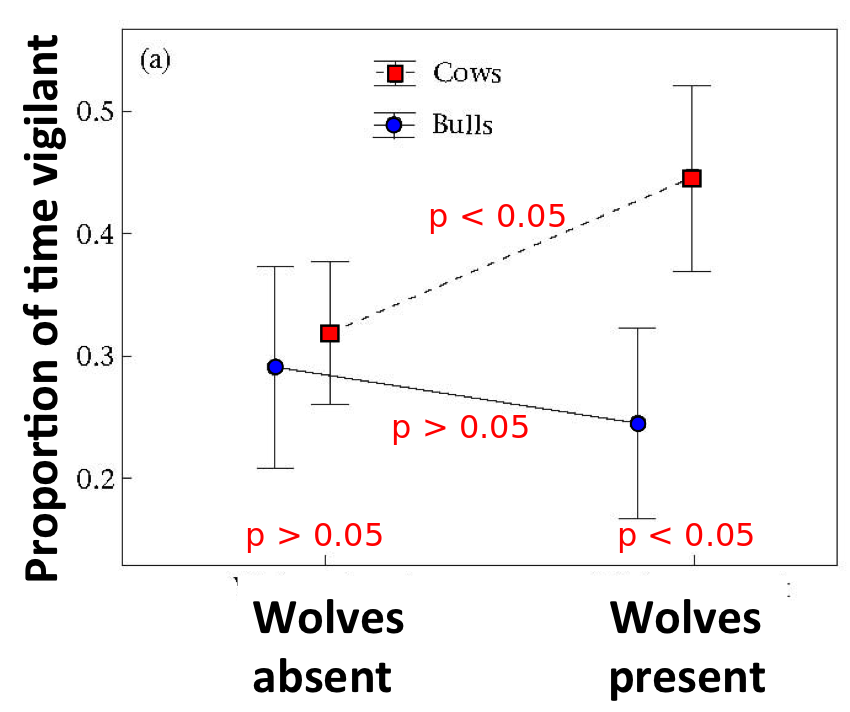
\includegraphics[width=\columnwidth]{elk-vigilance-sex.png}

        \end{columns}

    \end{adjustwidth}
\end{frame}
}

\section{How do prey respond to predators?}

\begin{frame}[t]
    \begin{adjustwidth}{-2em}{-1.5em}
        How do prey respond to predators?

        \vspace{2mm}
        \begin{enumerate}
            \item \textbf{Standing defenses} are always present

                \vspace{2mm}
                Examples: porcupine quills, camouflage in moths,
                chemical spray from skunks.
        \end{enumerate}

        \uncover<2->{
        Design an experiment to test the hypothesis that THC is
        an effective standing defense in \textit{Cannabis sativa}.

        \nbox{Need with-without design. Expose two lines of \textit{C. sativa}
            (one that lacks (or very low) THC and one with high levels of THC)
            to herbivores and measure rate of herbivory/growth rate/number of
            seeds produced.}
        }

    \end{adjustwidth}
    \note[item]{Getting eaten is really crummy for fitness; strong selection to
        avoid it}
\end{frame}

\begin{frame}[t]
    \begin{adjustwidth}{-2em}{-1.5em}

        \vspace{-2mm}
        \begin{enumerate}
            \addtocounter{enumi}{1}
            \item \textbf{Inducible defenses} are produced in response to
                predation (or presence of predators).

                \vspace{2mm}
                \uncover<2->{
                E.g., blue crabs (predator) and mussels (prey)
                }
        \end{enumerate}

        \begin{columns}

            \column{0.5\linewidth}

            \uncover<2->{
            Low predation of mussels in high tidal-flow areas; high predation
            in low-tidal flow areas.
            
            \vspace{8mm}
            Draw the bars you expect if shell thickness is an inducible defense
            }

            \column{0.5\linewidth}

            \includegraphics<2->[width=\columnwidth]{mussel-shell-axes.png}

        \end{columns}

    \end{adjustwidth}
\end{frame}

\begin{frame}[t]
    \begin{adjustwidth}{-2em}{-1.5em}

        \vspace{-2mm}
        \begin{enumerate}
            \addtocounter{enumi}{1}
            \item \textbf{Inducible defenses} are produced in response to
                predation (or presence of predators).

                \vspace{2mm}
                E.g., blue crabs (predator) and mussels (prey)
        \end{enumerate}

        \vspace{4mm}
        Predation rate is \textbf{correlated} with shell thickness. What are
        other reasonable hypotheses for the \textbf{cause} of thicker shells
        in high predation (low-tidal flow) areas?

        \nbox{Age differences---individuals in low-flow areas are older}
        \nbox{Selection---crabs have eaten thin-shelled individuals}
        \nbox{Differences in shell thickness is caused by the flow
            differences}
        \nbox{Differences in shell thickness is caused by other differences
            between low and high-flow areas (temperature, light, substrate,
            etc.)}
        \nbox{Genetic---mussels in low and high flow areas are genetically
            divergent, independent populations}

    \end{adjustwidth}
\end{frame}

\begin{frame}[t]
    \begin{adjustwidth}{-2em}{-1.5em}

        \vspace{-3mm}
        Hypothesis: Mussels increase shell thickness in response to evidence of
        predation.

        \vspace{2mm}
        Experimental test:

        \vspace{1mm}
        \nbox{In book (Figure 55.10); 2 treatments: (1) mussels downstream from
            crabs that are fed fish (NOT mussels!), and (2) mussels downstream
            from no crabs}

        \vspace{2mm}
        \nbox{If we want to test if mussels will increase shell thickness in
            response to evidence of predation, we need to adjust this
            experiment, so that the two treatments are (1) mussels downstream
            from broken mussel shells, and (2) mussels downstream from
            intact, but empty, mussel shells.}

    \end{adjustwidth}
\end{frame}

\clickerslide{
\begin{frame}
    \begin{clickerquestion}
        \item What are the costs and benefits of having an inducible defense
            against predators or herbivores?
    \end{clickerquestion}

    \begin{adjustwidth}{-2em}{-1.5em}
    \begin{table}%[htbp]
        \centering
        \begin{tabular}{ l | L{5.2cm} | L{5.2cm} | }
            \multicolumn{1}{c}{} &
            \multicolumn{1}{c}{Cost of inducible defense} &
            \multicolumn{1}{c}{Benefit of inducible defense} \\
            \cline{2-3}
            \textcolor{red}{1)} &
            Specialist consumers not deterred &
            Eliminates threat of predation \\
            \cline{2-3}
            \textcolor{red}{2)} &
            Generalist consumers not deterred &
            Flexible---many different types of defense are possible \\
            \cline{2-3}
            \textcolor{red}{3)} &
            Only effective for adults (not juveniles) &
            Effective at all life stages \\
            \cline{2-3}
            \textcolor{red}{4)} &
            \clickeranswer{Time lab---may be too late} &
            \clickeranswer{Don't invest resources unless needed} \\
            \cline{2-3}
        \end{tabular}
    \end{table}
    \end{adjustwidth}
\end{frame}
}

\section{How do predators affect communities of species?}

\begin{frame}[t]
    \begin{adjustwidth}{-2em}{-1.5em}
        How do predators affect communities of species?

        \vspace{4mm}
        A \textbf{keystone species} has an extraordinarily large impact on
        the surrounding community, relative to its abundance.

        \vspace{4mm}
        \uncover<2->{
        E.g. \spp{Pisaster} removal experiments

        \centerline{
        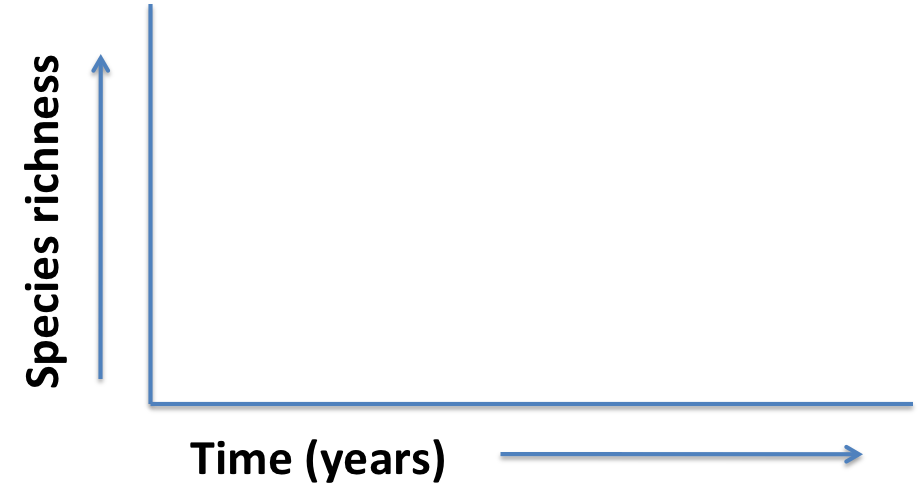
\includegraphics[height=0.5\textheight]{species-richness-axes.png}
        }
        }

    \end{adjustwidth}
    \note[item]{Go Dawgs! Pisaster = purple sea star. Tatoosh Island off tip of
        Olympic Peninsula.}
    \note[item]{Draw line for control plots (plots where Pistaster was not
        removed) = Stable at 15--18 species per meter plot.}
    \note[item]{In experimental plots, only one species left (California
        mussel).}
    \note[item]{Sea stars primary prey item is mussels}
    \note[item]{Sea star wasting disease (virus) all along Pacific Coast of
        North America}
\end{frame}

\clickerslide{
\begin{frame}
    \begin{clickerquestion}
        \item Which of the following is a valid conclusion to draw from
            these data? 

        \begin{clickeroptions}
            \item Mussels show induced defenses in the presence of
                \spp{Pisaster}. 
            \item \clickeranswer{Species richness is higher in the presence of
                    \spp{Pisaster} than in the absence of \spp{Pisaster}.}
            \item Mussels eliminate competing species by secreting a toxin.
                This toxin does not deter \spp{Pisaster}, however.  
            \item Mussels crowd out other species because they are superior
                competitors for space.
        \end{clickeroptions}
    \end{clickerquestion}
\end{frame}
}

\begin{frame}[t]
    \begin{adjustwidth}{-2em}{-1.5em}
        \vspace{-3mm}
        Trophic cascades in the Yellowstone Ecosystem

        \centerline{
        \includegraphics<1|handout:0>[height=0.7\textheight]{yellowstone-web-no-wolves.png}
        \includegraphics<2-|handout:1>[height=0.7\textheight]{yellowstone-web.png}
        }

        \uncover<3->{
        What's the impact of wolf reintroduction on birds of prey? Beaver?

        \nbox{Birds of prey increase due to decreased competition for rodent
            prey. Beaver increase due to decreased competition for resources =
            many more wetlands!}
        }

    \end{adjustwidth}
\end{frame}

\section{Why is the world green?}

\begin{frame}[t]
    \begin{adjustwidth}{-2em}{-1.5em}
        Why is the world green?

        \begin{itemize}
            \item[$H_1$:]<2-> Top-down control hypothesis

                \nbox{Herbivore populations are limited by consumers (predators
                    and parasites)}

                \vspace{8mm}
            \item[$H_2$:]<3-> Poor-nutrition hypothesis (N-limitation)---on a
                per-gram basis, plants contain $<$10\% of N found in animals.

                \nbox{Herbivore populations are limited by N available in plants}

                \vspace{8mm}
            \item[$H_3$:]<4-> Plant defense hypothesis 

                \vspace{2mm}
                E.g., Nicotine as an inducible defense
        \end{itemize}
    \end{adjustwidth}
    \note[item]{Be able to design an experiment that would test the top-down
        and poor-nutrition hypotheses}
\end{frame}

\begin{frame}[t]
    \begin{adjustwidth}{-2em}{-1.5em}
        Nicotine as an inducible defense
        
        \vspace{6mm}
        Synthesized in roots in response to attack by herbivores and transported
        to trichomes (``leaf hairs'')

        \uncover<2->{
        \vspace{6mm}
        Experiment: Study 3 populations of wild tobacco. For many generations,
        each has been exposed to different levels of herbivory (low, medium,
        and high).
        }

        \uncover<3->{
        \begin{enumerate}
            \item Grow individuals from each population in the same environment

                \vspace{2mm}
            \item Induce nicotine production in each (same stimulus)

                \vspace{2mm}
            \item Measure nicotine production and the number of seeds produced
        \end{enumerate}
        }

    \end{adjustwidth}
\end{frame}

\begin{frame}[t]
    \begin{adjustwidth}{-2em}{-1.5em}
        \vspace{-3mm}
        Data on average number of seeds produced per plant:

        % \vspace{2mm}
        \begin{table}%[htbp]
            \centering
            \begin{tabular}{ | L{3.5cm} | C{2cm} | C{2cm} | }
                \multicolumn{1}{c}{Source population} &
                \multicolumn{1}{c}{Induced} &
                \multicolumn{1}{c}{Not induced} \\
                \hline
                Low herbivory & 4494 & 6047 \\[2ex]
                Medium herbivory & 5314 & 7335 \\[2ex]
                High herbivory & 4860 & 4705 \\
                \hline
            \end{tabular}
        \end{table}

        \vspace{2mm}
        NOTE: Individuals from all three populations show about the same
        response to induction (same nicotine production).

    \end{adjustwidth}
\end{frame}

\clickerslide{
\begin{frame}[t]
    \begin{adjustwidth}{-2em}{-1.5em}
        \vspace{-3mm}
        Data on average number of seeds produced per plant:

        % \vspace{2mm}
        \begin{table}%[htbp]
            \centering
            \begin{tabular}{ | L{3.5cm} | C{2cm} | C{2cm} | }
                \multicolumn{1}{c}{Source population} &
                \multicolumn{1}{c}{Induced} &
                \multicolumn{1}{c}{Not induced} \\
                \hline
                Low herbivory & 4494 & 6047 \\[2ex]
                Medium herbivory & 5314 & 7335 \\[2ex]
                High herbivory & 4860 & 4705 \\
                \hline
            \end{tabular}
        \end{table}

        \begin{clickerquestion}
            \item Which of the following is a valid conclusion to draw from
                these data?
            \begin{clickeroptions}
                \item Whether induced or not, seed production is lower in
                    populations that are normally exposed to herbivores.  
                \item \clickeranswer{After induction, seed production is
                        reduced in the low and medium herbivory populations,
                        but not in the high herbivory population.}
                \item There is a ``cost of defense'' in all three of these
                    populations.   
                \item There is no ``cost of defense'' in populations exposed to
                    medium levels of herbivory (they produce the largest number
                    of seeds).
            \end{clickeroptions}
        \end{clickerquestion}

    \end{adjustwidth}
\end{frame}
}


\end{document}

\clickerslide{
\begin{frame}
    \begin{clickerquestion}
        \item 
        \begin{clickeroptions}
            \item 
            \item 
            \item 
            \item 
        \end{clickeroptions}
    \end{clickerquestion}
\end{frame}
}

\clickerpost{
{
\usebackgroundtemplate{\includegraphics[page=17,width=\paperwidth]{./24-Radiation-extinction.pdf}}
\begin{frame}[t,plain]
    \begin{adjustwidth}{-2em}{-1.5em}
        \cmask{Answer: 3}
    \end{adjustwidth}
\end{frame}
}
}

